\documentclass[11pt]{article}
\usepackage[utf8]{inputenc}
\usepackage{enumitem}
\usepackage{graphicx}
\usepackage{xcolor}
\title{CSE-476: Introduction to Natural Language Processing}
\date{}
\begin{document}
\begin{center}
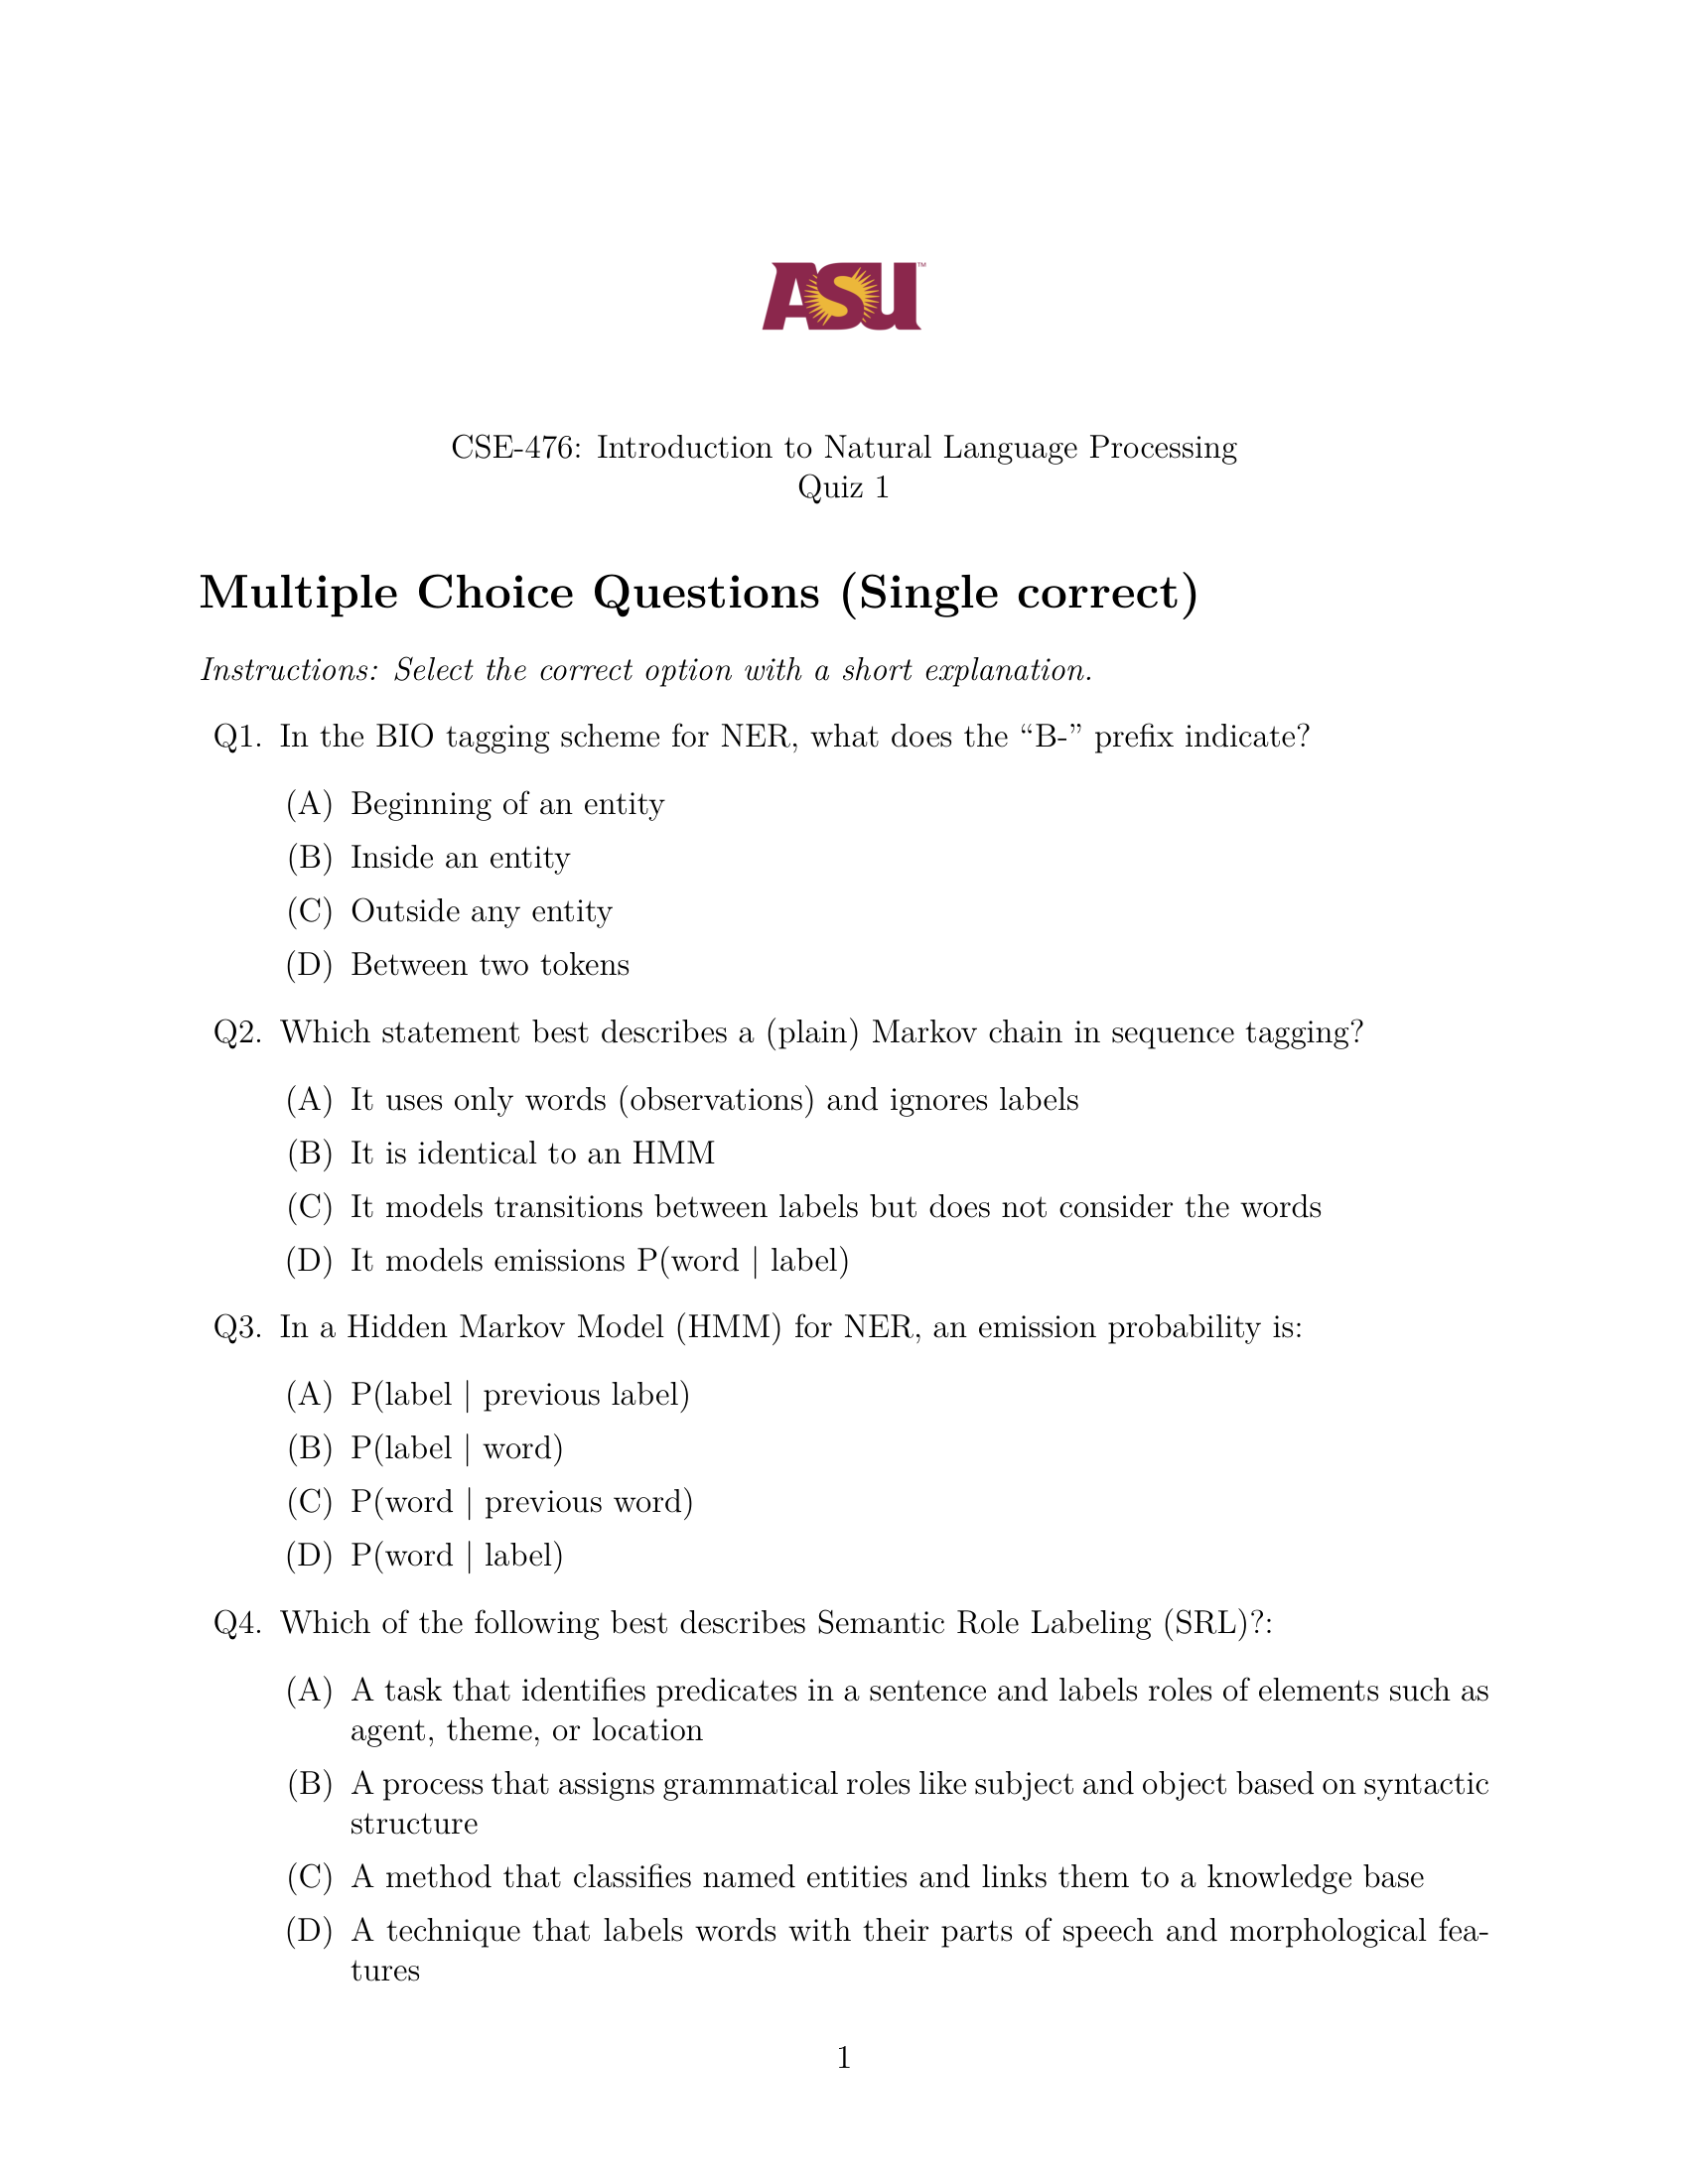
\includegraphics[width=0.2\textwidth]{page_images/page_1.png}

CSE-476: Introduction to Natural Language Processing\\
Quiz 1
\end{center}

\bigskip

\textbf{\Large Multiple Choice Questions (Single correct)}

\medskip

\textit{Instructions: Select the correct option with a short explanation.}

\medskip

Q1. In the BIO tagging scheme for NER, what does the ``B-'' prefix indicate?

\begin{itemize}
\item[(A)] Beginning of an entity
\item[(B)] Inside an entity
\item[(C)] Outside any entity
\item[(D)] Between two tokens
\end{itemize}

Q2. Which statement best describes a (plain) Markov chain in sequence tagging?

\begin{itemize}
\item[(A)] It uses only words (observations) and ignores labels
\item[(B)] It is identical to an HMM
\item[(C)] It models transitions between labels but does not consider the words
\item[(D)] It models emissions $P(\text{word} \mid \text{label})$
\end{itemize}

Q3. In a Hidden Markov Model (HMM) for NER, an emission probability is:

\begin{itemize}
\item[(A)] $P(\text{label} \mid \text{previous label})$
\item[(B)] $P(\text{label} \mid \text{word})$
\item[(C)] $P(\text{word} \mid \text{previous word})$
\item[(D)] $P(\text{word} \mid \text{label})$
\end{itemize}

Q4. Which of the following best describes Semantic Role Labeling (SRL)?:

\begin{itemize}
\item[(A)] A task that identifies predicates in a sentence and labels roles of elements such as agent, theme, or location
\item[(B)] A process that assigns grammatical roles like subject and object based on syntactic structure
\item[(C)] A method that classifies named entities and links them to a knowledge base
\item[(D)] A technique that labels words with their parts of speech and morphological features
\end{itemize}

\begin{center}
1
\end{center}

\clearpage

Q5. Which of the following best describes Byte Pair Encoding (BPE)?

\begin{enumerate}[(A)]
\item A technique that compresses text by replacing consecutive repeated characters with a count and a symbol
\item A tokenization method that iteratively merges the most frequent pair of symbols in a corpus
\item A tokenization method that splits text based on whitespace and punctuation
\item A character-level encoding scheme that assigns fixed-length binary codes to characters
\end{enumerate}

Q6. Which of the following best describes the main goal of tokenization in NLP?

\begin{enumerate}[(A)]
\item To label each token with a grammatical category
\item To convert text into a sequence of symbols suitable for modeling
\item To reduce vocabulary size to zero
\item To assign probabilities to sentences
\end{enumerate}

Q7. Why is splitting text by spaces (text.split(" ")) considered an insufficient tokenizer?

\begin{enumerate}[(A)]
\item It produces too many tokens
\item It does not work well for languages without explicit word boundaries
\item It cannot tokenize English at all
\item It ignores punctuation entirely
\end{enumerate}

Q8. Which of the following is NOT listed as a common sequence tagging task?

\begin{enumerate}[(A)]
\item Part-of-speech tagging
\item Named Entity Recognition
\item Dependency parsing
\item Sentiment analysis
\end{enumerate}

Q9. What is a common limitation of BIO tagging for Named Entity Recognition?

\begin{enumerate}[(A)]
\item It cannot represent overlapping or nested entities
\item It requires too many labels
\item It does not support multiple entity types
\item It ignores entity boundaries
\end{enumerate}

\begin{center}
2
\end{center}

\clearpage

Q10.\ When choosing between character-level tokenization and sentence-level tokenization,\\
which trade-off must be considered?

\medskip

\hspace*{2em}(A) Speed vs accuracy

\hspace*{2em}(B) Tokenized sequence length vs vocabulary size

\hspace*{2em}(C) Precision vs recall

\hspace*{2em}(D) Memory vs computation

\vfill

\textit{End of Paper}

\begin{center}
3
\end{center}
\end{document}